

\chapter{Design}
\label{ch:design}
The design of the project consists of three individual elements, that are then combined to produce a resulting application. This approach has been chosen to allow us to focus independently on what each section needs as per our requirements. It also permits us to ignore any integration till further in the project, ensuring that each individual element works as expected before moving on to the next.

These three elements have been identified as the: Emulator, Visualisation and Module System. These three encapsulate the entirety of the project into our three individual sections, with the Emulator and Visualisation making the core of the project, whilst the Module System being a later addition to the project to allow for easier implementation of additional modules, and also satisfying requirements \ref{req:md} and \ref{req:fp} to include the Multiply and Divide, and Single Precision Floating Point Module


\begin{figure}[h]
    \centering
    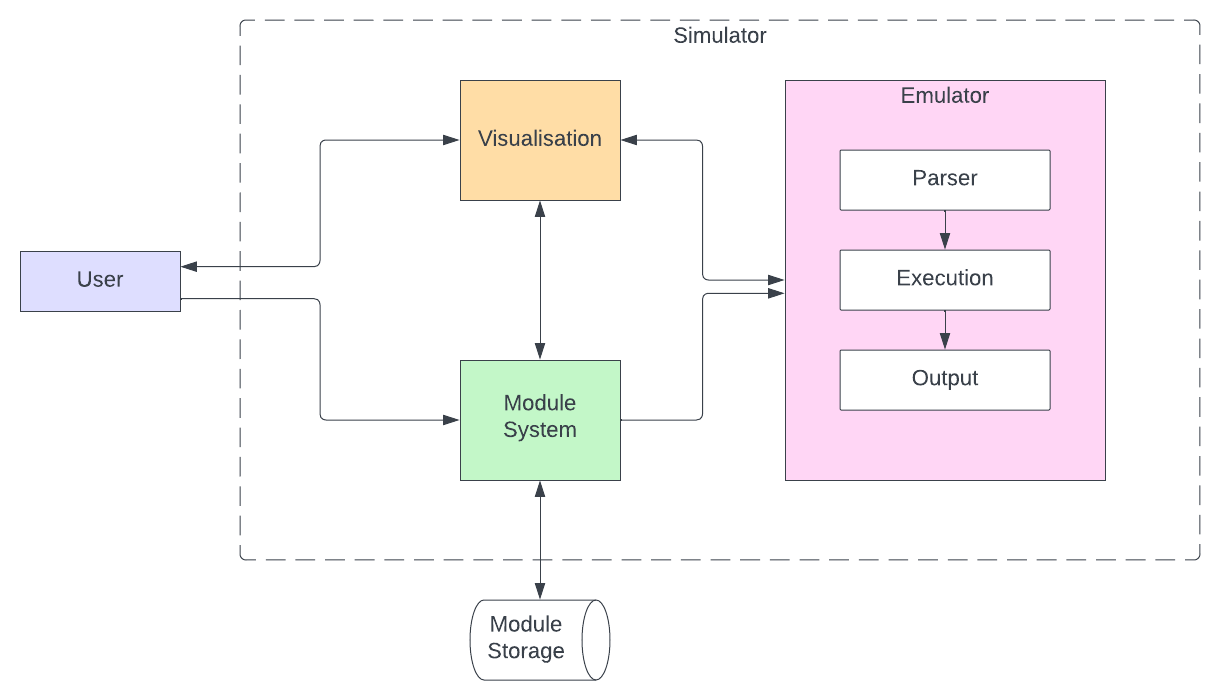
\includegraphics[width=0.95\linewidth]{dissertation/DATA/sys architecture.png}
    \caption{Overall System Architecture}
    \label{fig:sys_architecture}
\end{figure}

Each of the three systems integrates tightly with the other as seen in the system architecture diagram in Figure \ref{fig:sys_architecture}. At the core the Emulator links directly with the visualisation and module system, with the module and visualisation directly connected as we aim for modules to be able to modify the UI directly, as well as providing new features for emulation. We also note a Hard Disk storage for modules, this is the case as these must persist over application runs, and will remain locally on the users device. Our visualisation denotes the end user interface that will be built in JavaFX with the emulator being created from scratch in Java.

It is important to consider how a user may interact with the system in everyday use. A depiction of a typical user flow can been seen in the sequence diagram in Figure \ref{fig:user_sequence}. It covers how a user may enter code, have the system emulate and visualise, show error feedback for invalid code and how a user may go about enabling or disabling a module of choice.

\begin{figure}[h]
    \centering
    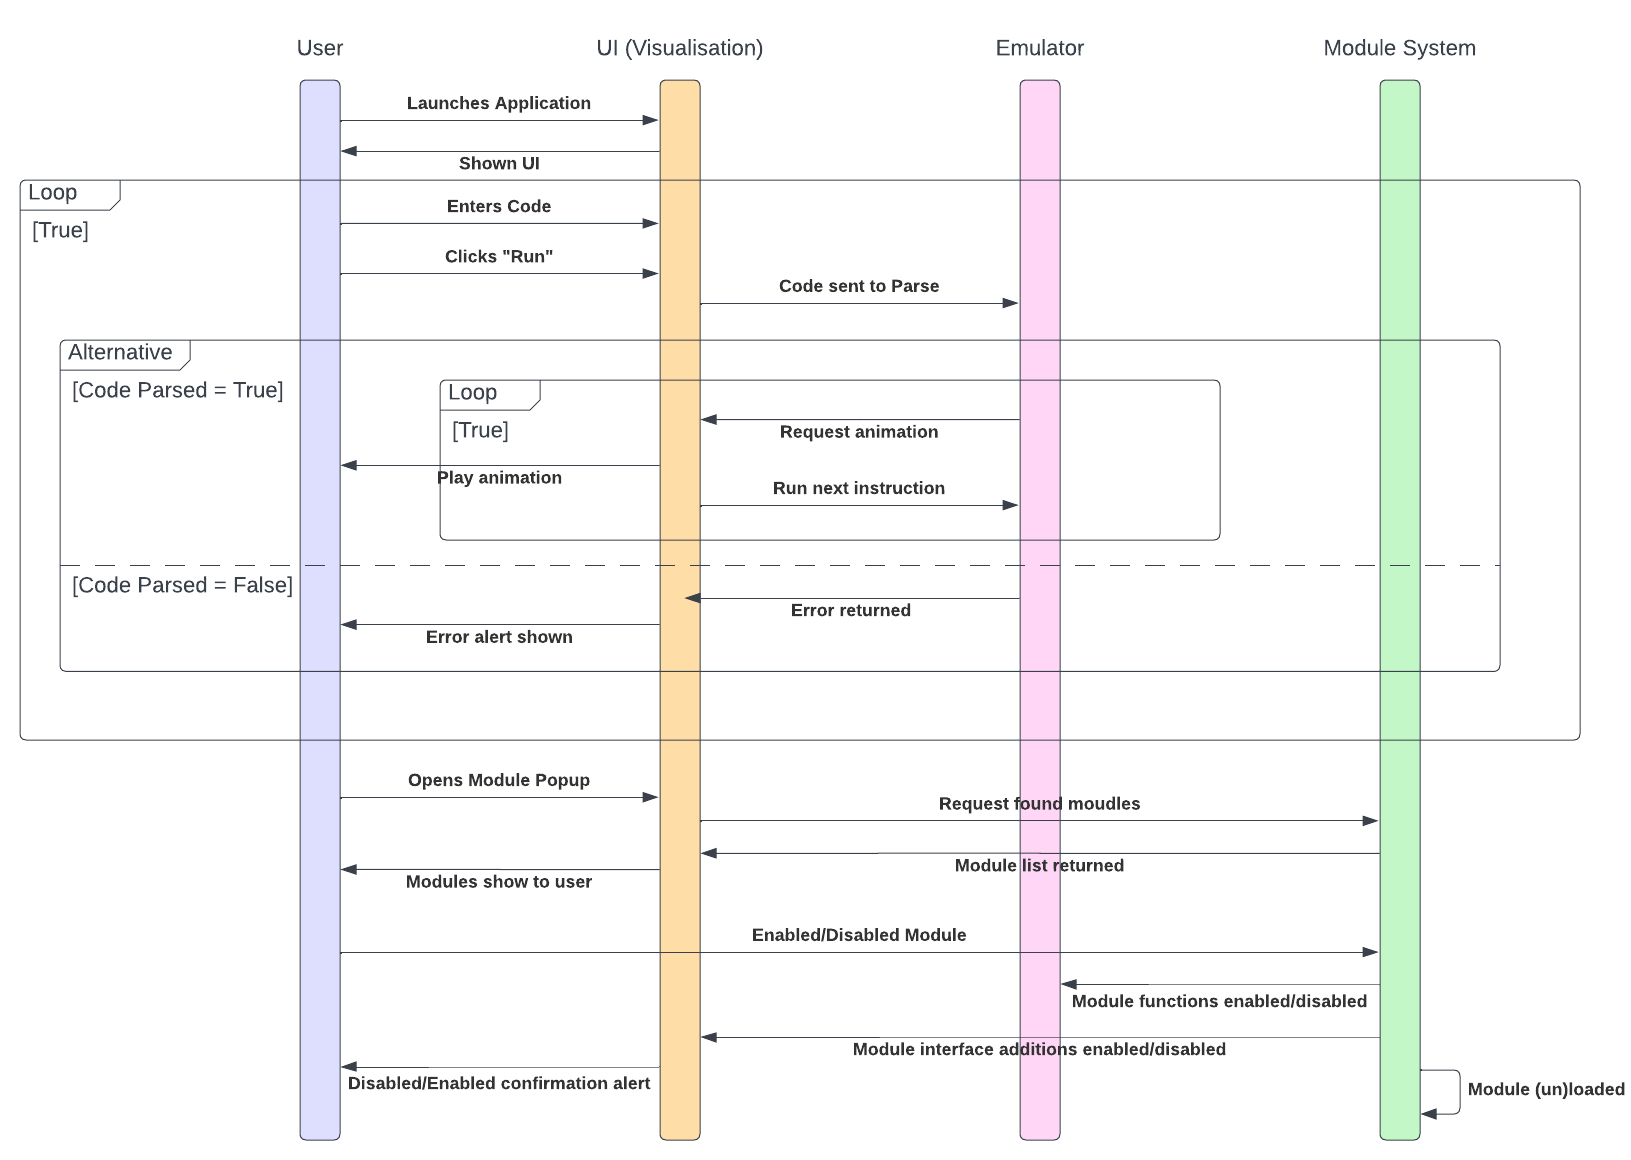
\includegraphics[width=0.95\linewidth]{dissertation/DATA/sequence diagram.png}
    \caption{Example user sequence diagram}
    \label{fig:user_sequence}
\end{figure}

\section{Emulator}
The emulator is designed to mock the RISC-V architecture closely, whilst also being simple and efficient.

At its core we have an Instruction class that will encapsulate each individual RISC-V instructions logic with individual isntructions being stored centrally and referenced by name. This will exist as a abstract class, with common code already present, but explicitly providing an \verb|execute()| method to be implemented by sub-classes, containing the relevant code to emulate the respective RISC-V instruction. 

In Figure \ref{fig:instr_abstract_uml} we denote a simple example of the ADD instruction implementing the Abstract Instruction class and overriding the \verb|execute()| method.

\begin{figure}[H]
    \centering
    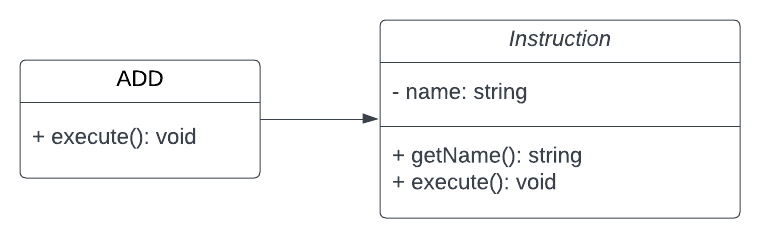
\includegraphics[width=0.95\linewidth]{dissertation/DATA/instr_abstract_uml.png}
    \caption{Basic UML diagram of the Abstract instruction class}
    \label{fig:instr_abstract_uml}
\end{figure}

There also needed to be a consideration on how the emulator will represent memory and register values. In both cases, a 32 bit value needs to be stored. This could simply be stored as a string of 32$\times$1's and 0's or as a 32 bit integer type in Java. However, a custom binary representation was chosen as it make operations simpler (Figure \ref{fig:bin_regmem_uml}), providing a simple interface to read and write the value as binary, denary or hex. This allowed the emulator to have a consistency between memory and registers without having to transform values between the two.

Within our registers we need to be able to hold the 32 base registers, with the ability to reference them by not only their name, but also their respective Application Binary Interface name as well \cite{riscvinternational_2014_calling}(page 3) which is an alternate name denoting specific usage or idea placement of data. Thus a map would work best to map the string name and application binary interface name to a register object.

Similarly memory needs to be addressable by its 4 byte aligned location, and thus we could opt for two methods of referencing:
\begin{enumerate}
    \item Use a list and take modulo 4 of addressed to get the relative index in the list for each memory value.
    \item Use a map to store the location as a key, with the memory value as the value, avoiding extra computation to calculate locations.
\end{enumerate}
Both are valid options. However, option 2 provides the benefit of a O(1) lookup time, compared to O(n) for a list, and seeing as the memory may become infinitely large with a complex emulation, option 2 suffices as the better choice.

Figure \ref{fig:bin_regmem_uml} shows a example of the design of our Binary object, with it being utilised by both our \texttt{Register} and \texttt{MemoryValue}'s, which in turn have a class that contains the reference to each register/memory value that can be used by the system. In our design it should note the similarity between Memory and Registers, and that this is something that could be refactored into an interface, or generic class in the future.

\begin{figure}[H]
    \centering
    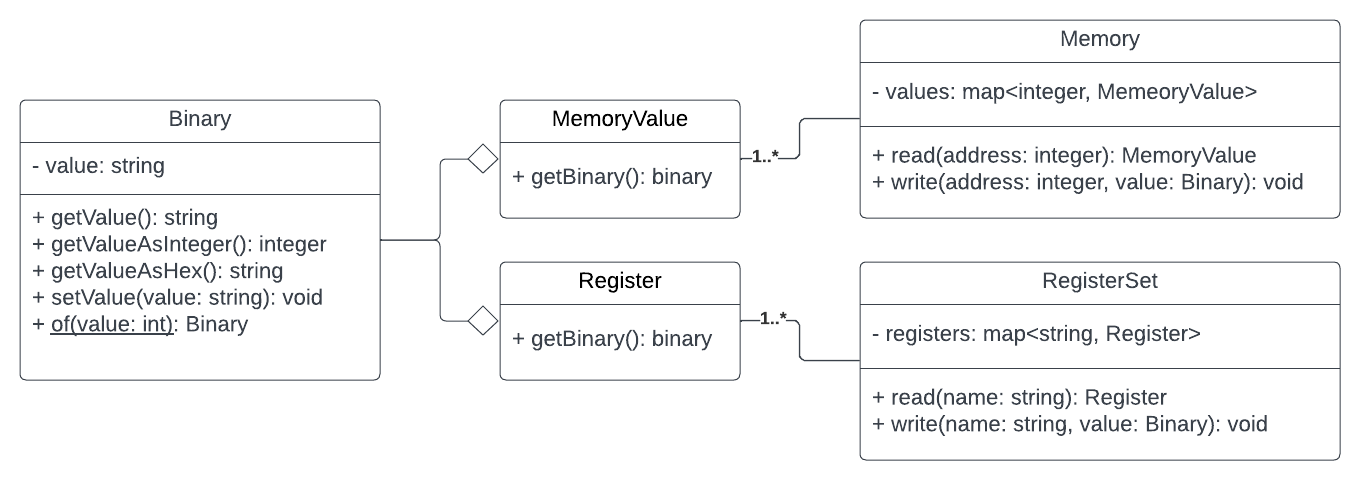
\includegraphics[width=\linewidth]{dissertation/DATA/bin_regmem_uml.png}
    \caption{Binary, Memory and Register UML Diagram}
    \label{fig:bin_regmem_uml}
\end{figure}

In order to emulate any given code, it needs to be parsed into our designed instruction system via a parser. The parser should be efficient and simple, providing suitable error feedback when required.

The parser is designed to consume a user program line-by-line. Each line is expected to conform to a valid instruction with operands. For example the following valid ADDI instruction will read register x1, add 3 to it and then write it back to register x1:\\\\
\verb|ADDI x1, x1, 3|
\\\\
The parser should first identify the instruction from its name, and then identify how many operands it should have and of what type they should be. In the ADDI example above, it should have 3 operands of type: REGISTER, REGISTER and IMMEDIATE. 

Only when the written instructions has the matching amount of operands and respective types should it be accepted and transformed into our instruction format to be run later.

In the event of a parse error, an error will be raised and parsing will stop and the raised error will be passed back up to the UI for the user to see. Each parse error will be specific and clear as to the issue, and will include a line error to help reference the correct instruction in the program. On a complete successful parse, the transformed program should be passed onto the rest of the emulator to be executed as noted in thew system architecture in Figure \ref{fig:sys_architecture}.

\section{Visualisation}
The visualisation of the emulation is a large part of the project, with the overall simulation relying heavily on a well designed UI.

\begin{figure}[H]
    \centering
    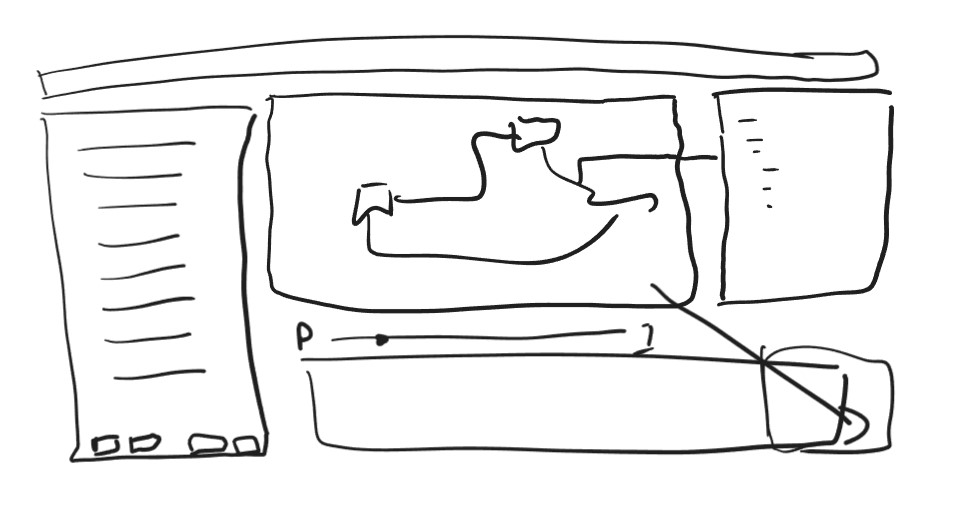
\includegraphics[width=\linewidth]{dissertation/DATA/early_design.jpg}
    \caption{Original hand drawn UI design}
    \label{fig:early_ui_design}
\end{figure}

Our first UI design (Figure \ref{fig:early_ui_design}) was designed to be simple, and loosely based on the design of LittleManComputer (Figure \ref{fig:lmc}) and Emulsiv (Figure \ref{fig:emulsiv}) as discussed in Section \ref{sec:lmc} and \ref{sec:emulsiv} respectively. 
The design places the code editor on the left, the main visualisation area in the centre, registers on the right, memory along the bottom and a menu bar stretching the top. These positions were specifically chosen based on the constraint of element sizing:
\begin{itemize}
    \item The code editor requires a large vertical space to hold many lines of code, but a relatively short horizontal width, due to the average instruction being relatively short.
    \item The animation/visualisation area was given the most space as this is the main focus point of the application, and thus being dead centre is the most appropriate location within the UI.
    \item Registers, much like the code editor require a small horizontal space to display their value, but 32 of them need to be on display at any given time, thus a large horizontal space allows for this with minimal scrolling on smaller screens.
    \item Memory also requires limited horizontal space, however, unlike registers, it starts of empty for every execution, and may not be used in any given execution, thus designating it to the bottom to fill waste space is more appropriate. Should the memory fill up, the user may scroll through it to see all the values at any given time.
\end{itemize}

As-well as the overall \ac{UI} design, a simple yet intuitive layout needed to be created to visualise the internal data movement around the processor components (Arithmetic Logic Unit, Control Unit, Instruction Register, Instruction Decoder, Instruction Memeory, Registers and Memory). The original design of this can be seen below in Figure \ref{fig:early_animation_design} with, Control Unit designs in Figure \ref{fig:early_cu_design}.

\begin{figure}[H]
    \centering
    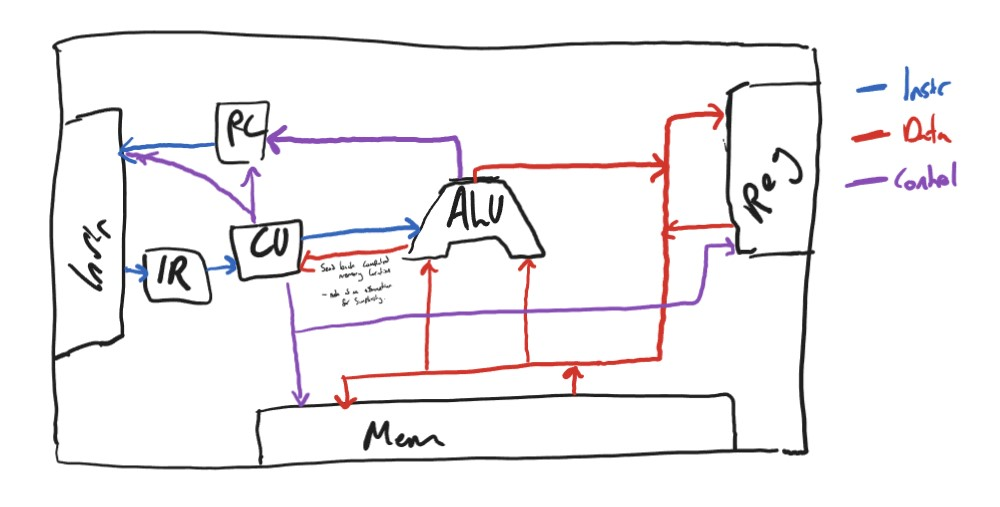
\includegraphics[width=\linewidth]{dissertation/DATA/animation_layout.jpg}
    \caption{Original animation area design}
    \label{fig:early_animation_design}
\end{figure}

\begin{figure}[H]
    \centering
    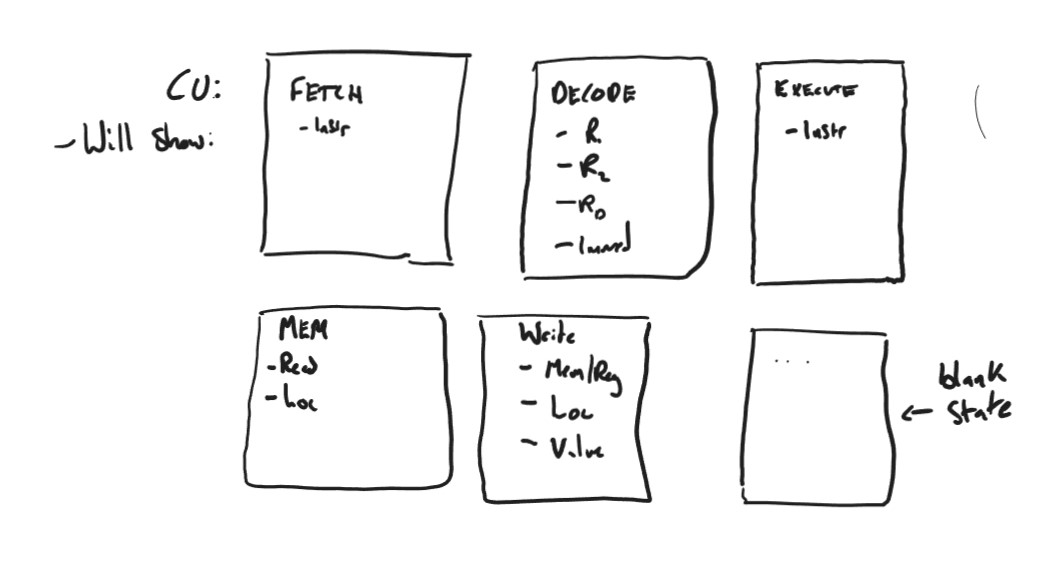
\includegraphics[width=\linewidth]{dissertation/DATA/control_unit.jpg}
    \caption{Original Control Unit design}
    \label{fig:early_cu_design}
\end{figure}

\begin{figure}[H]
    \centering
    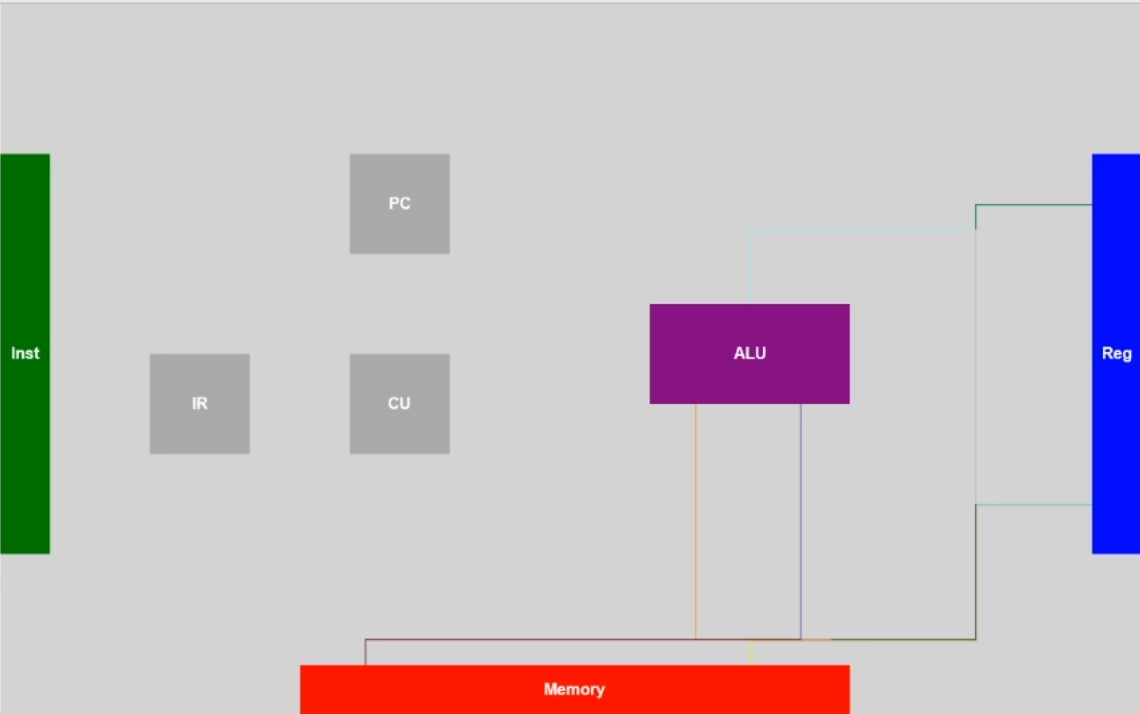
\includegraphics[width=0.9\linewidth]{dissertation/DATA/first_design_implementation.jpg}
    \caption{Implemented design based on sketches}
    \label{fig:origina_implemented_design}
\end{figure}

With these hand drawn designs, we can produce a full mock up design in JavaFX with the first implementation as seen in Figure \ref{fig:origina_implemented_design} above.

UI Designs should be easy to use for all users, and should follow common and practised design principles. Nielsen's Heuristics \cite{nielsen_2020_10} denote 10 usability principles to improve and grade UI design. Our design satisfies some of the principles, but not all. Principal 1 and 8 relate to visibility of system status and aesthetic and minimalist design. 

With our current design we pose an issue of visibility to users that suffer from colourblindness, or visual impairments, which in-turn makes the design un-aesthetic for them. The choice of red, green and blue for the Memory, Instructions and Registers was originally decide to help them stand out, however, these may appear as a murky brown to colourblind users, and they further draw attention away from the core aspect of the visual area. The choice of background colour is also poor here, with a darkish gray background with darker gray boxes on top, producing a low contrast between these elements. The Web Accessibility Initiative \cite{webaccessibilityinitiativew3_2022_understanding} denotes a minimum contrast ratio of 4.5:1, which they gray on gray does not provide. Further the currently drawn example line are far too thin, and may be missed by users with visual impairments.

To rectify these issues, several changes were made to the design including:
\begin{enumerate}
    \item Lightening of the background to increase the contrast ration to an acceptable level,
    \item Convert the red, green and blue boxes to grayscale to alleviate the issue for colourblind users,
    \item Switch the gray boxes to purple, and convert the ALU into its more familiar shape to conform with principle 4 (Consistency and Standards) as to match with other simulators and diagrams.
    \item Lines were made thicker to ensure they are easier to see, and the red lines in the original design were switched to black
\end{enumerate}

With these changes visible in the second implementation of the design in Figure \ref{fig:second_implemented_design}

\begin{figure}[H]
    \centering
    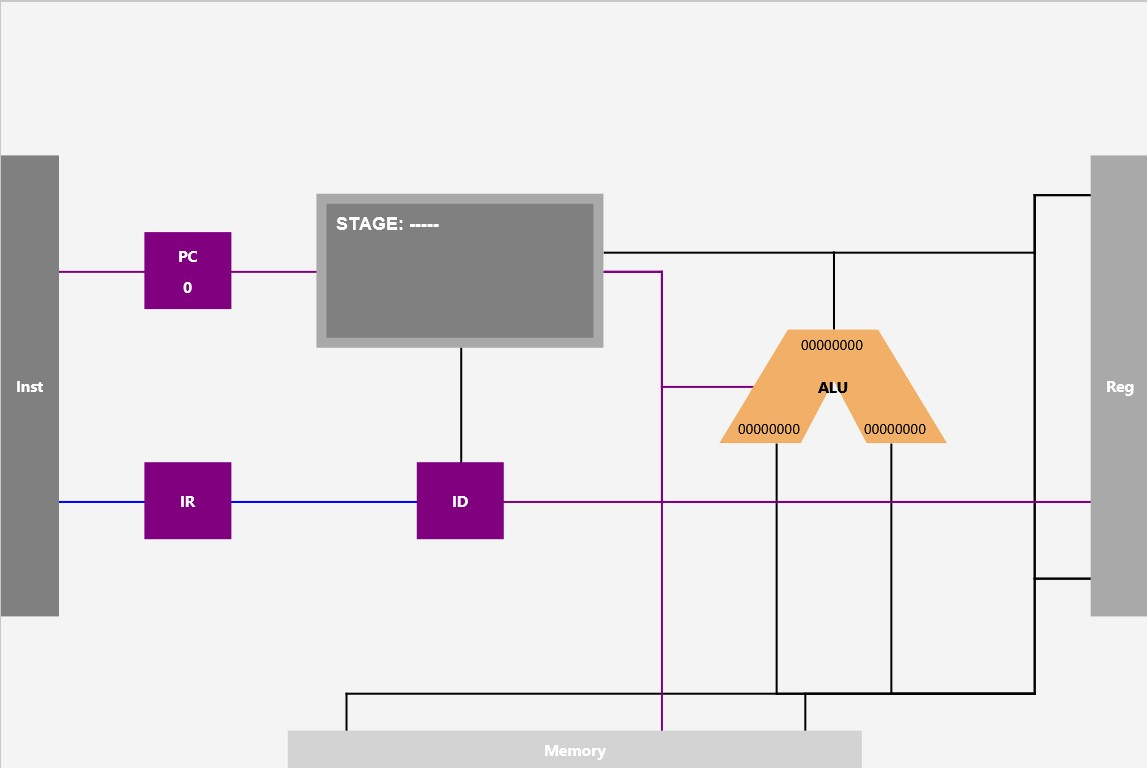
\includegraphics[width=0.9\linewidth]{dissertation/DATA/second_design_implementation.jpg}
    \caption{Re-implemented design with usability changes and principles taken into account}
    \label{fig:second_implemented_design}
\end{figure}

This newer design also includes an example of a fleshed out Control Unit, with space for information to be included later, and a bold white font to state the current stage of execution.

The final design ended up matching closely with our original hand drawn designs, and can be seen in Figure \ref{fig:final_implemented_design}. It wraps the registers and memory values into two tables, that can be resized by the end user to focus on different representations of values, as well as allowing for more or less values to be present at any given time. This end design also provides a large amount of responsiveness, with each major area being re-sizeable from being completely hidden, to taking up the entire screen, with each section dynamically adjusting in real-time. This resulting design most importantly follows Nielsen's 8th principle, with a simple and minimalist design, with only whats required on screen, and further principle 4, keeping our layout and design consistent across the entire application.

\begin{figure}[H]
    \centering
    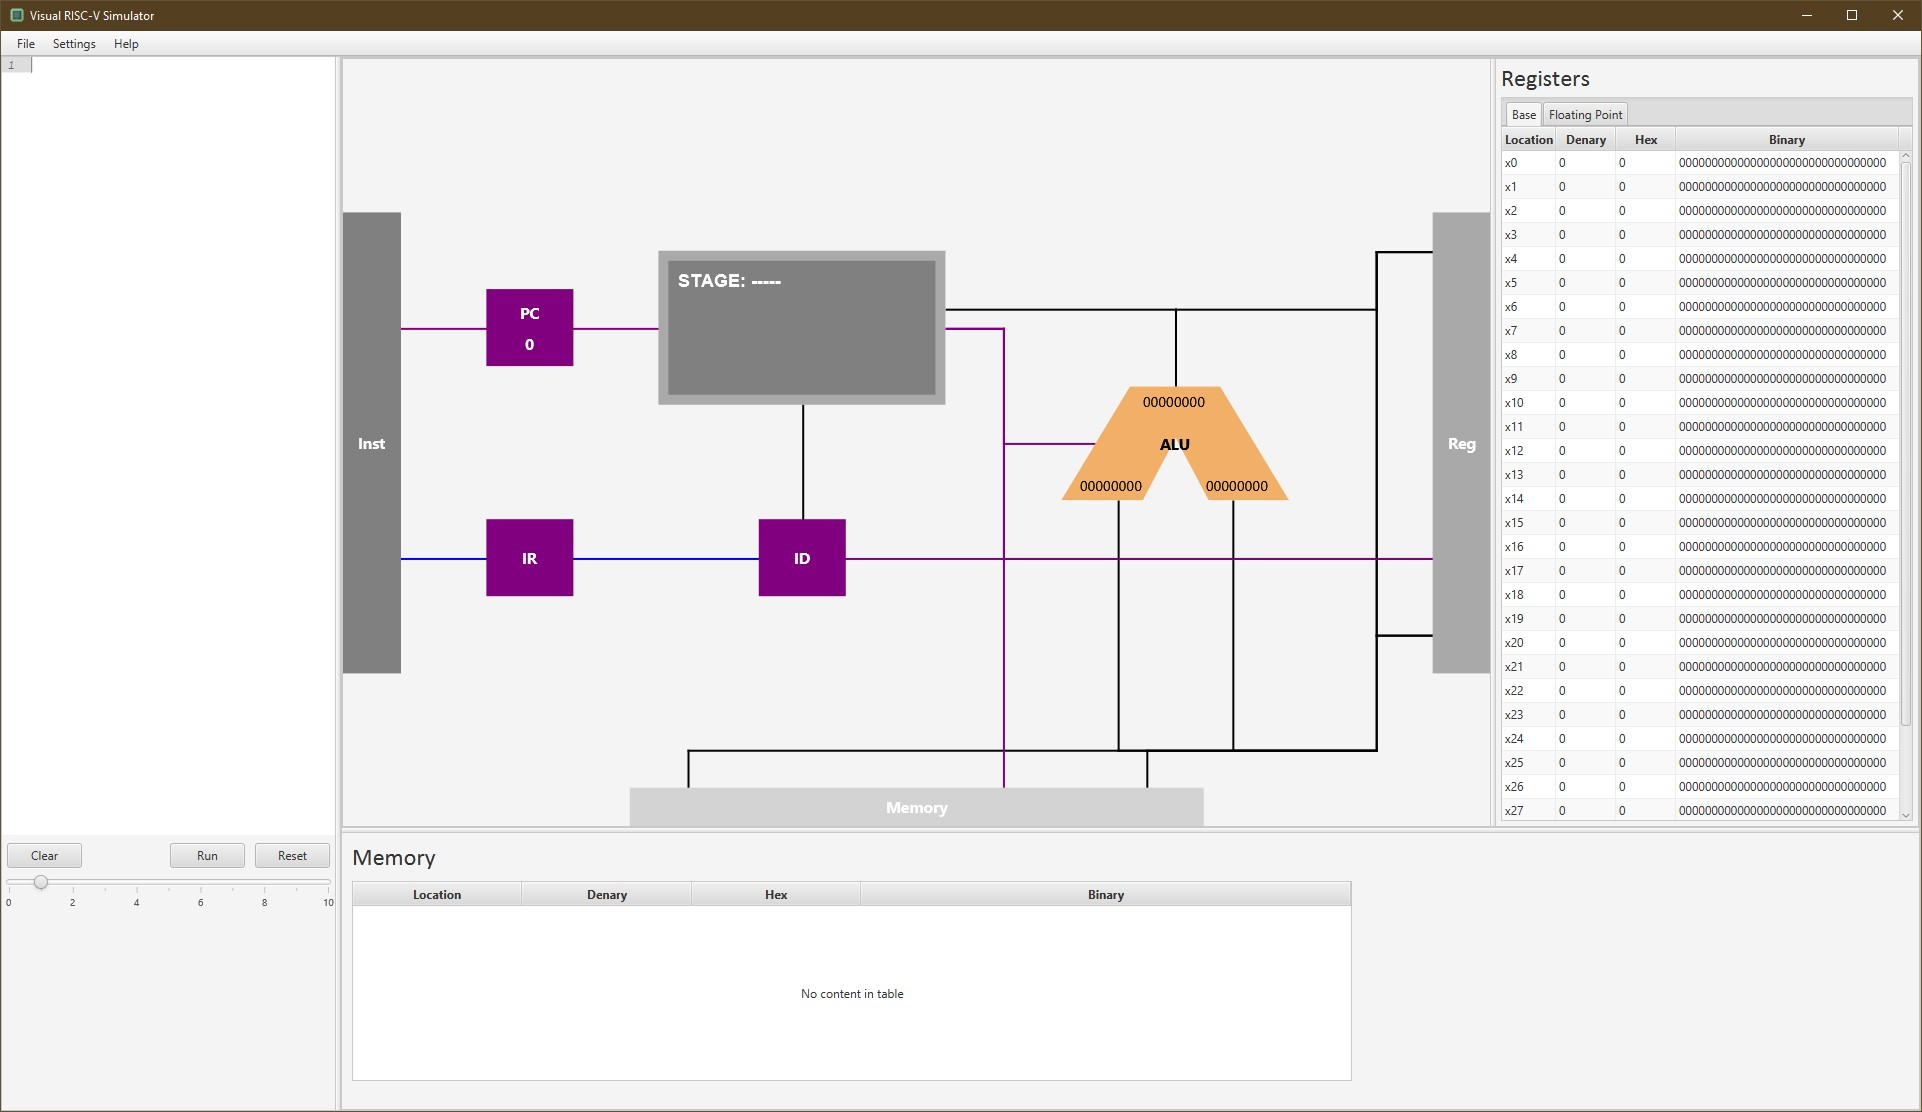
\includegraphics[width=0.9\linewidth]{dissertation/DATA/final_design.jpg}
    \caption{Final full UI design}
    \label{fig:final_implemented_design}
\end{figure}

\subsection{Differences from Specification}
In the specification (Appendix ...) MaterialFX \cite{palexdev_2022_palexdevmaterialfx} was discussed to re-skin (re-theme) the application to provide a more modern feel, matching styling that is commonly found online. However, due to a lack of skin's (A skin is a collection of styles that are applied to a given element to change the way it looks) for more advanced elements, MaterialFX was not used, in favour of using the default skin for JavaFX components, as once fully implemented, the mismatch of differently skinned components looked convoluted and made the UI somewhat confusing to use.

\section{Module System}
The applications module system is designed to be convenient and intuitive to use.

\begin{figure}[H]
    \centering
    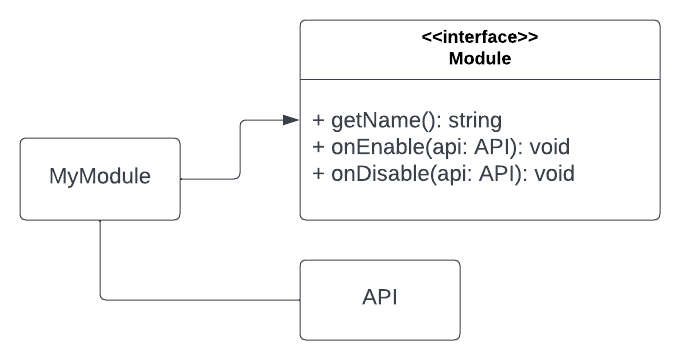
\includegraphics[width=0.9\linewidth]{dissertation/DATA/module uml.png}
    \caption{Module System UML Diagram}
    \label{fig:module_uml}
\end{figure}

Modules are designed to implement a simple module interface (Figure \ref{fig:module_uml}). This can then be identified by the system and loaded at run time, allowing a module to incorporate any custom logic as required. This basic design also permits users to write their own modules to extend the system within the constraints of the module systems API.

With this design each module should implement and override the respective functions, and then make use of the provided API in order to extend functionality, without directly interfacing with the core code. This adds a layer of protection, limiting module access to ensure that modules don't break core functionality or attempt to inject malicious code.

\subsection{Design modifications}
The project design had to be altered slightly to permit the addition of modules. Our emulator design required no changes to facilitate module design, as per our design our instructions are stored centrally, and new instructions can be simply registered with this central store at any point in time to be used.

On the visualisation side, a few changes had to be made:

\begin{enumerate}
    \item An extra tab was added to the design to allow opening of a module popup,
    \item A module popup (Figure \ref{fig:module_popup_design}) was designed to facilitate the enabling and disabling of modules, as-well as the ability to add and remove additional modules,
    \item The register area was adapted to permit multiple register views, in the form of panes that can be clicked through (This can bee seen in Figure \ref{fig:final_implemented_design})
\end{enumerate}

\begin{figure}[H]
    \centering
    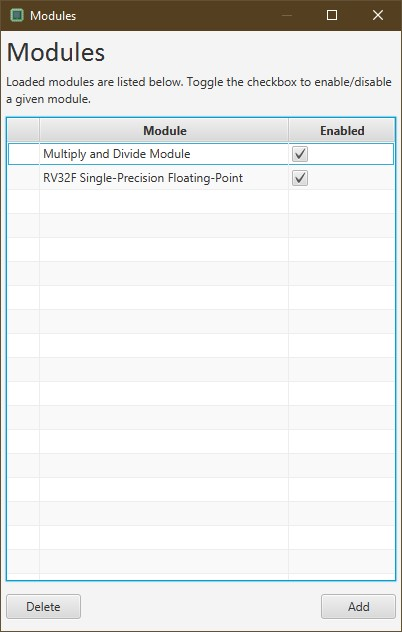
\includegraphics[width=0.4\linewidth]{dissertation/DATA/module_popup.jpg}
    \caption{Module Popup implemented design}
    \label{fig:module_popup_design}
\end{figure}
